% =============================================================================
% PART B - MODULE 44-45: AI CONTENT MODERATION \& FACE SCAN
% In Charge: Pham Kha Vy
% =============================================================================
\subsection{Module 44--45: AI Content Moderation \& Face Scan}

\subsubsection{M44.01 -- Moderate Content by AI (UC-46.01)}
\begin{itemize}[leftmargin=1.5em,itemsep=2pt]
  \item \textbf{Screen Name \& Route Path:} Create Post Modal -- \texttt{/forum/\{categorySlug\}}.
  \item \textbf{Who Can Use This:} Client, Freelancer, AI System.
  \item \Needspace{6\baselineskip}\textbf{Before You Begin:} User is creating a new forum post.
\end{itemize}
\begin{figure}[H]\centering
  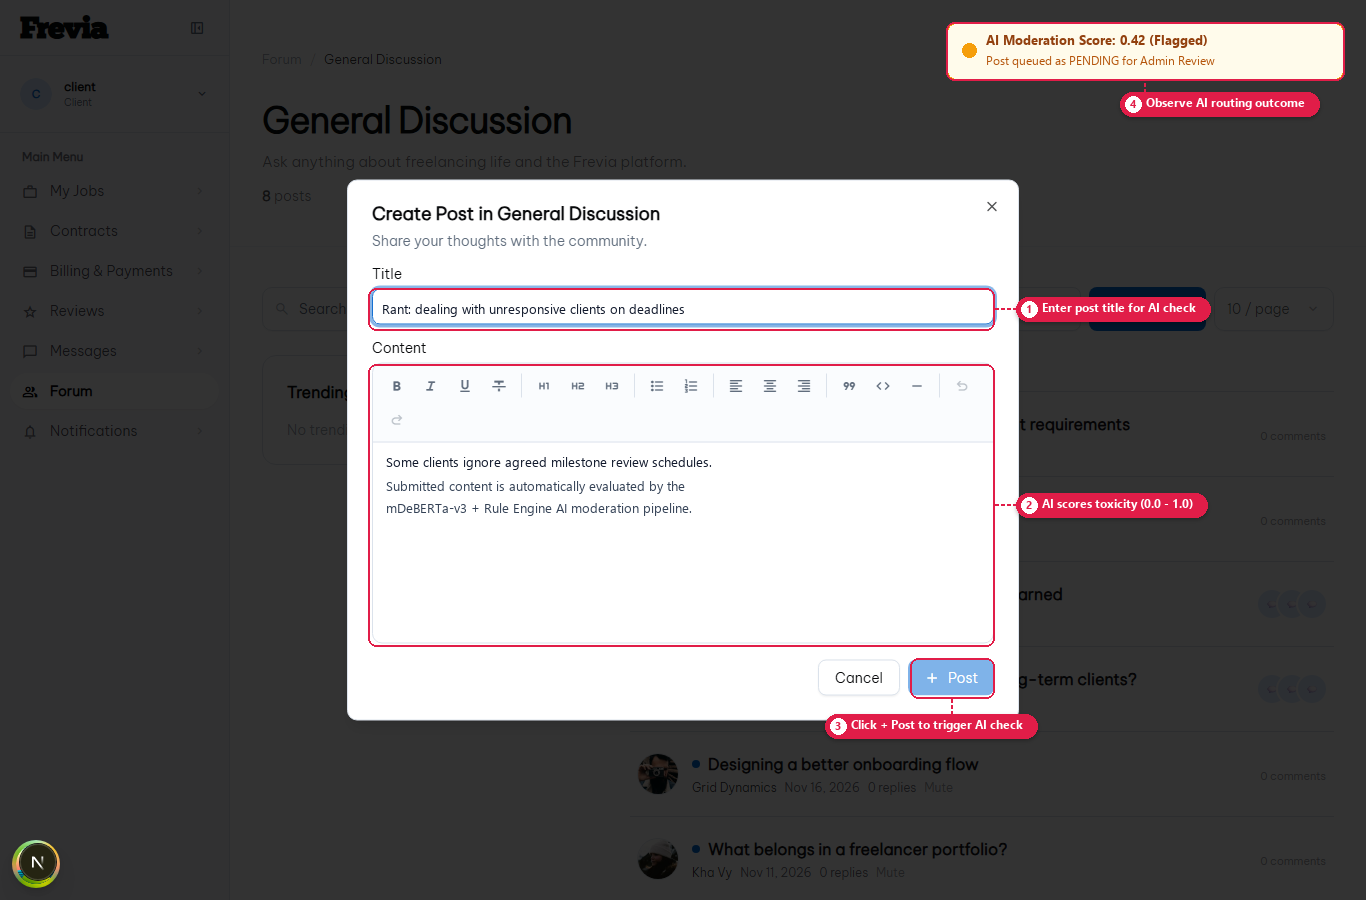
\includegraphics[width=0.90\textwidth]{images/ai/ai_moderate_guide.png}
  \caption{AI Content Moderation scoring during post creation}
\end{figure}
\Needspace{6\baselineskip}\paragraph{Step-by-Step User Guide:}
\begin{enumerate}[leftmargin=1.8em,itemsep=3pt]
  \item \rbadge{1} \textbf{Enter Post Title:} Type your post title in the \textbf{Create Post} dialog.
  \item \rbadge{2} \textbf{Compose Content for AI Scoring:} Write your post body; upon submission, the AI service computes a toxicity score from 0.0 to 1.0.
  \item \rbadge{3} \textbf{Submit Post:} Click \textbf{+ Post} to run the automated FastAPI content moderation pipeline.
  \item \rbadge{4} \textbf{Observe AI Routing Outcome:} Review the live toast notification: score $<0.3$ publishes immediately; $0.3$--$0.8$ queues as \texttt{PENDING} for Admin Moderation; $\ge 0.8$ is blocked.
\end{enumerate}
\Needspace{6\baselineskip}\paragraph{After You Submit (Result \& Troubleshooting):}
\begin{itemize}[leftmargin=1.5em,itemsep=2pt]
  \item \textbf{What Happens Next:} Safe content goes live instantly while borderline content is routed to Admin Moderation.
  \item \textbf{Troubleshooting \& Common Messages:} Posts scoring $\ge 0.8$ return HTTP 400 with a policy violation alert and are not stored.
\end{itemize}

\subsubsection{M45.01 -- Scan Face and Detect Duplicate Identity (UC-47.01)}
\begin{itemize}[leftmargin=1.5em,itemsep=2pt]
  \item \textbf{Screen Name \& Route Path:} Profile \& Trust Settings (Identity Tab) -- \texttt{/freelancer/profile}.
  \item \textbf{Who Can Use This:} Freelancer, Expert, AI System.
  \item \Needspace{6\baselineskip}\textbf{Before You Begin:} Prepare clear CCCD front/back photos and allow browser camera access.
\end{itemize}
\begin{figure}[H]\centering
  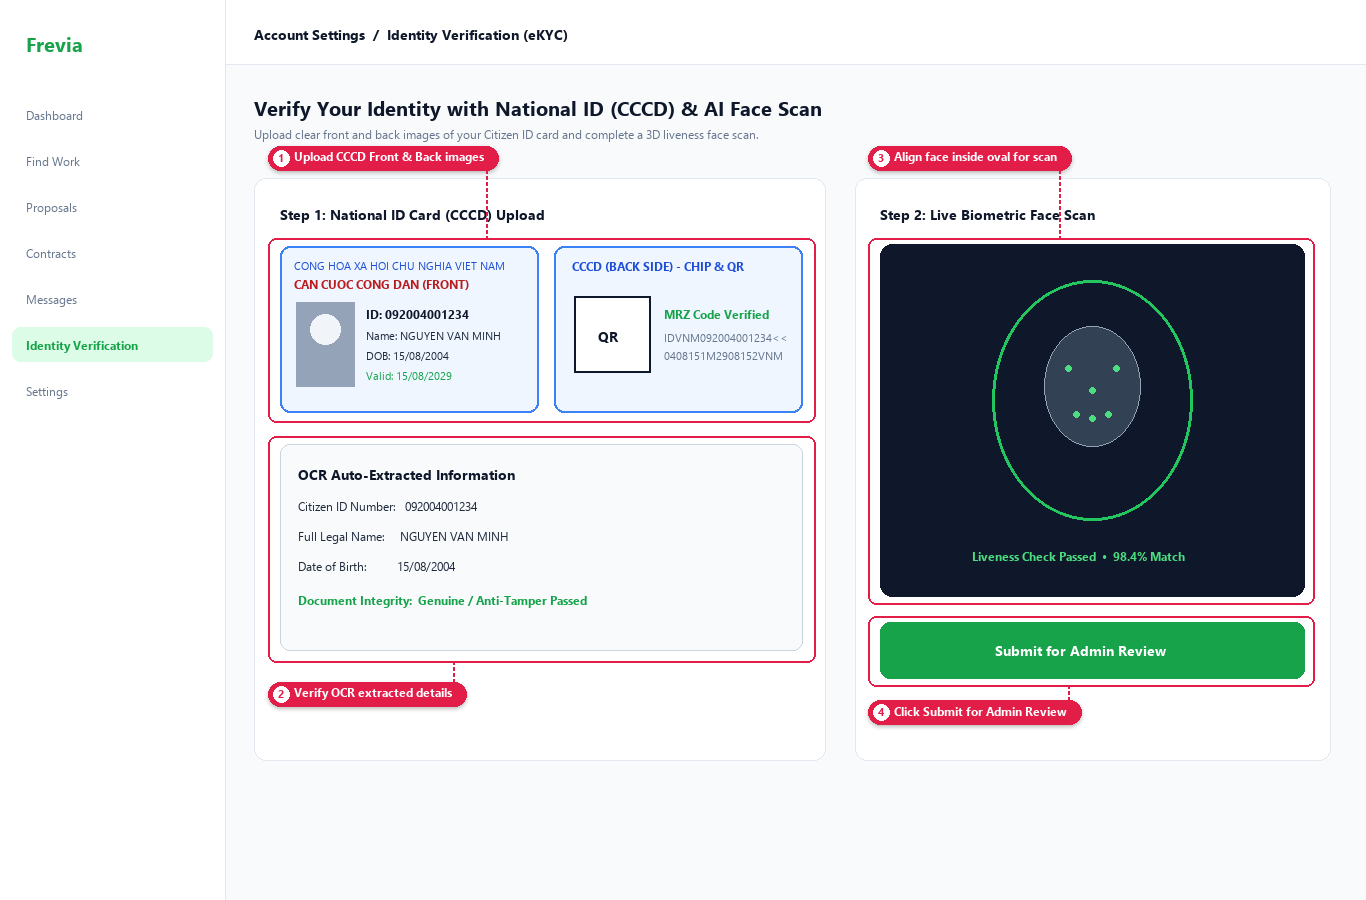
\includegraphics[width=0.90\textwidth]{images/ai/ai_face_scan_guide.png}
  \caption{User Guide: Profile Identity Tab -- CCCD Upload and Live AI Liveness Face Scan}
\end{figure}
\Needspace{6\baselineskip}\paragraph{Step-by-Step User Guide:}
\begin{enumerate}[leftmargin=1.8em,itemsep=3pt]
  \item \rbadge{1} \textbf{Upload CCCD Front \& Back:} Select \textit{National ID card} and upload clear photos for \textit{ID card front} and \textit{ID card back} (JPG/PNG/WEBP, max 10\,MB each).
  \item \rbadge{2} \textbf{Align Face in Live Camera:} Click \textbf{Start liveness check}, grant camera access, and keep your face centered inside the live AI camera frame.
  \item \rbadge{3} \textbf{Complete 3-Pose Liveness Prompts:} Follow the on-screen prompts (\textit{1. Look straight}, \textit{2. Turn left}, \textit{3. Turn right}) until \textit{Liveness check completed} appears.
  \item \rbadge{4} \textbf{Submit for AI Verification:} Click the blue \textbf{Submit for AI verification} button to run AI OCR, anti-spoofing, and duplicate face matching before final Admin approval.
\end{enumerate}
\Needspace{6\baselineskip}\paragraph{After You Submit (Result \& Troubleshooting):}
\begin{itemize}[leftmargin=1.5em,itemsep=2pt]
  \item \textbf{What Happens Next:} Extracted identity data and facial match scores are stored with duplicate-check flags.
  \item \textbf{Troubleshooting \& Common Messages:} Blurry documents or duplicate ID/face matches trigger an alert for manual review.
\end{itemize}

